\documentclass[10pt, oneside]{article} 
\usepackage{amsmath, amsthm, amssymb, calrsfs, wasysym, verbatim, bbm, color, graphics, graphicx, geometry, tocloft, subcaption, blindtext, hyperref}

\geometry{tmargin=.75in, bmargin=.75in, lmargin=.75in, rmargin = .75in}  

\newcommand{\R}{\mathbb{R}}
\newcommand{\C}{\mathbb{C}}
\newcommand{\Z}{\mathbb{Z}}
\newcommand{\N}{\mathbb{N}}
\newcommand{\Q}{\mathbb{Q}}
\newcommand{\Cdot}{\boldsymbol{\cdot}}

% comment command
\newcommand{\Comment}[1]{\noindent \textcolor{blue}{\textit{#1}} \par}

\newtheorem{thm}{Theorem}
\newtheorem{defn}{Definition}
\newtheorem{conv}{Convention}
\newtheorem{rem}{Remark}
\newtheorem{lem}{Lemma}
\newtheorem{cor}{Corollary}

\setlength{\parindent}{0pt}


\title{Security \& Cryptography Class Notes}
\author{Anna Visman}
\date{Academic Year 2024-2025}

\begin{document}

\maketitle
\tableofcontents

\vspace{.25in}

\section{Lecture 1}

\subsection{Security Overview}

A computer system is said to be secure if it satisfies the following properties:
\begin{itemize}
\item {\bf Confidentiality}: Unauthorized entities cannot access the system or its data
\item {\bf Integrity}: When you receive data, it is the right one
\item {\bf Availability}: The system or data is there when you need it
\end{itemize}

\begin{rem}
The mere presence of these properties does not necessarily mean that the system is fully secure in practice.
\end{rem}

A secure system is reliable:

\begin{itemize}
    \item Keep your personal data confidential 
    \item Allow only authorised access or modifications to resources
    \item Ensure that any produced results are correct
    \item Give you correct and meaningful results whenever you want them
\end{itemize}


Terminology:

\begin{itemize}
    \item {\bf{Assets}}: Things we want to protect (hardware, software, data)
    \item {\bf{Vulnerabilities}}: Weaknesses in a system that may be exploited in order to cause loss and harm
    \item {\bf{Threats}}: A loss or harm that might befall a system (interception, interruption, modification, fabrication)
    \item {\bf{Attack}}: An action which exploits a vulnerability to execute a threat 
    \item {\bf{Control/Defence}}: Removing/reducing a vulnerability. You control a vulnerability to prevent an attack and defend against a threat
\end{itemize}

Methods of Defence:

\begin{itemize}
    \item Prevent it
    \item Deter it: make the attack harder or more expensive
    \item Deflect it: make yourself less attractive to attacker
    \item Detect it: notice that the attack is occurring
    \item Recover from it: mitigate the effects of the attack
\end{itemize}

Principle of Easiest Penetration: A system is only as secure as its weakest link. An attacker will go after whatever part of the system is easiest for them, not most convenient for you. In order to build secure systems, we need to learn how to think like an attacker!

\subsection{Defense Overview}
Software controls:
\begin{itemize}
    \item Passwords and other forms of access control
    \item Operating systems separate users' actions from each other
    \item Virus scanner watch for malware
    \item Development controls enforce quality measures on the original source code 
    \item Personal firewalls that run on your desktop
\end{itemize}

Hardware controls:
\begin{itemize}
    \item Not usually protection of the hardware itself, but rather using separate hardware to protect the system as a whole 
    \item Fingerprint readers
    \item Smart tokens
    \item Firewalls
    \item Intrusion detection systems
\end{itemize}

Physical Systems:
\begin{itemize}
    \item Protection of the hardwell itself, as well as physical access to the console, storage media, etc.
    \item Locks
    \item Guards
    \item Off-site backups
\end{itemize}

Policies and Procedures:
\begin{itemize}
    \item Non-technical means can be used to protect against some classes of attack (e.g. VPNs for accessing interal company network)
    \item Rules about choosing Passwords
    \item Training in best security practices
\end{itemize}

\subsection{Cryptography Overview}
Objectives of Cryptography:
\begin{itemize}
    \item Protecting data privacy
    \item Authenticaion (message, data origin, entity)
    \item Non-repudiation: preventing the sender from later denying that they sent the message
\end{itemize}

\newpage

\begin{defn}
Kerkhoff's Principle: The adversary knows all details about a crypto system except the secret key.
\end{defn}

\begin{defn}
Cipher: A method or algorithm used to transform readable data (called plaintext) into an unreadable format (called ciphertext) to protect its confidentiality.
\end{defn}

Encryption is the process of converting plaintext into ciphertext. Decryption is the reverse process. Encryption uses the key k, decryption uses the key k'. If k = k', the system is symmetric. If k $\neq$ k', the system is asymmetric. Decryption(Encryption(m)) = m.
\begin{figure}[h!]
    \centering
    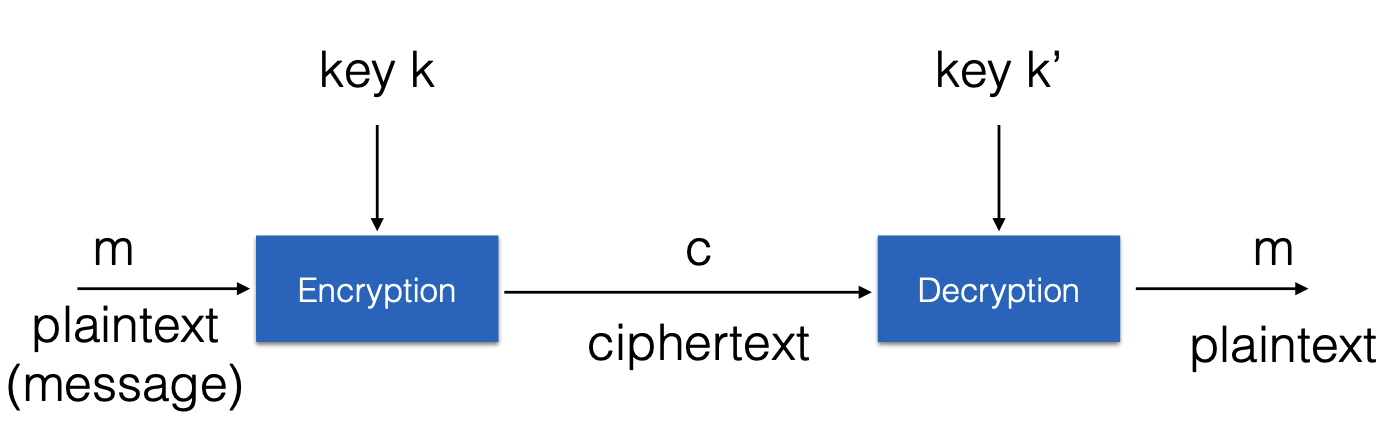
\includegraphics[scale=0.5]{img/w1encryption.png}
    \caption{Encryption}
\end{figure}

\begin{table}[h!]
    \centering
    \begin{tabular}{|l|l|l|}
    \hline
    \textbf{Feature}        & \textbf{Private Key Encryption}        & \textbf{Public Key Encryption}         \\ \hline
    \textbf{Keys}           & Same key for encryption \& decryption  & Two keys: public and private           \\ \hline
    \textbf{Speed}          & Faster                                 & Slower                                 \\ \hline
    \textbf{Key sharing}    & Must be kept secret                    & Only the private key is secret         \\ \hline
    \textbf{Use cases}      & Encrypting large data, e.g., files     & Secure key exchange, digital signatures \\ \hline
    \end{tabular}
    \caption{Summary of Differences Between Private and Public Key Encryption}
    \label{tab:encryption_comparison}
    \end{table}
    
\subsection{Topics Covered in Course}
\begin{itemize}
\item Classical systems: simple ciphers, substitution, permutation, transposition, Caesar, Vigenere
\item Information Theoretic Security
\item Defining security: pseudorandomness, one-way functions, trapdoor functions
\item Notions of security: perfect secrecy, semantic security, IND security
\item Attacks on encryption schemes: objective, levels of computing power, amount of information available
\item Types attacks: ciphertext-only, known plaintext, chosen plaintext, chosen ciphertext, adaptive
\item Different types of adversaries: unbounded/polynomial computing power
\item Security: unconditionally secure, computationally secure
\item and more... see slides
\end{itemize}


\section{Lecture 2}

\newcommand{\floor}[1]{\left\lfloor #1 \right\rfloor}

\subsection{Number Theory}

\subsubsection{Modular Arithmetic}
\begin{defn}
A positive integer \( N \) is called the \emph{modulus}. Two integers \( a \) and \( b \) are said to be congruent modulo \( N \), written \( a \equiv b \pmod{N} \), if \( N \) divides \( b - a \).
\end{defn}    

Examples:
\[
18 \equiv 4 \pmod{7}, \quad -18 \equiv 3 \pmod{7}.
\]

The set of integers modulo \( N \) is denoted by \( \mathbb{Z}/N\mathbb{Z} \) or \( \mathbb{Z}_N \):
\[
\mathbb{Z}/N\mathbb{Z} = \{ 0, 1, \dots, N-1 \}, \quad \#(\mathbb{Z}/N\mathbb{Z}) = N.
\]

Properties of Modular Arithmetic:
\begin{enumerate}
    \item Addition is closed: \(\forall a, b \in \mathbb{Z}/N\mathbb{Z} : a + b \in \mathbb{Z}/N\mathbb{Z}\).
    \item Addition is associative: \(\forall a, b, c \in \mathbb{Z}/N\mathbb{Z} : (a + b) + c = a + (b + c)\).
    \item \(0\) is an additive identity: \(\forall a \in \mathbb{Z}/N\mathbb{Z} : a + 0 = 0 + a = a\).
    \item The additive inverse always exists: \(\forall a \in \mathbb{Z}/N\mathbb{Z} : a + (N - a) = (N - a) + a = 0\).
    \item Addition is commutative: \(\forall a, b \in \mathbb{Z}/N\mathbb{Z} : a + b = b + a\).
    \item Multiplication is closed: \(\forall a, b \in \mathbb{Z}/N\mathbb{Z} : a \cdot b \in \mathbb{Z}/N\mathbb{Z}\).
    \item Multiplication is associative: \(\forall a, b, c \in \mathbb{Z}/N\mathbb{Z} : (a \cdot b) \cdot c = a \cdot (b \cdot c)\).
    \item \(1\) is a multiplicative identity: \(\forall a \in \mathbb{Z}/N\mathbb{Z} : a \cdot 1 = 1 \cdot a = a\).
    \item Multiplication and addition satisfy the distributive law: \(\forall a, b, c \in \mathbb{Z}/N\mathbb{Z} : (a + b) \cdot c = a \cdot c + b \cdot c\).
    \item Multiplication is commutative: \(\forall a, b \in \mathbb{Z}/N\mathbb{Z} : a \cdot b = b \cdot a\).
\end{enumerate}

\subsubsection{Modular Exponentiation}
Modular exponentiation is a technique used to efficiently compute expressions of the form \( a^b \mod m \), especially for large \( b \). The key idea is to repeatedly square the base \( a \), reduce modulo \( m \) at each step, and combine results as needed. \\

\textbf{Example: Compute \( 3^4 \mod 11 \)}

\begin{enumerate}
    \item Write the problem:
    \[
    3^4 \mod 11
    \]
 
 \item Break it into smaller steps using properties of modular arithmetic:
 \begin{enumerate}
    \item First, compute \( 3^2 \mod 11 \):
    \[
    3^2 = 9 \quad \Rightarrow \quad 9 \mod 11 = 9
    \]
    \item Then, square the result to get \( 3^4 \mod 11 \):
    \[
    3^4 = (3^2)^2 = 9^2 = 81 \quad \Rightarrow \quad 81 \mod 11 = 4
    \]
 \end{enumerate}
 
 \item Final result:
    \[
    3^4 \mod 11 = 4
    \]
 
\end{enumerate}
 
\textbf{General Algorithm: Exponentiation by Squaring}
\begin{enumerate}
    \item If \( b \) is even:
    \[
    a^b \mod m = \left( a^{b/2} \mod m \right)^2 \mod m
    \]
    \item If \( b \) is odd:
    \[
    a^b \mod m = \left( a \cdot a^{b-1} \mod m \right) \mod m
    \]
\end{enumerate}

You can also simplify the problem by reducing the base modulo:
\begin{defn}
    For any a, b, n, if $a \equiv b \pmod{n}$, then $a^k \equiv b^k \pmod{n}$ for any positive integer k.
\end{defn}
See an example of this in practice session 1 exercise 1e. 

\subsubsection{Groups and Rings}
\begin{defn}
    A \emph{group} is a set with an operation that is:
    \begin{itemize}
        \item Closed,
        \item Has an identity element,
        \item Associative, and
        \item Each element has an inverse.
    \end{itemize}
    \end{defn}
    
    \begin{defn}
    A group is \emph{abelian} if it is also commutative.
    \end{defn}
    
    Examples:
    \begin{itemize}
        \item The integers under addition (\( \mathbb{Z}, + \)), where the identity is \( 0 \) and the inverse of \( x \) is \( -x \).
        \item The nonzero rationals under multiplication (\( \mathbb{Q}^*, \cdot \)), where the identity is \( 1 \) and the inverse of \( x \) is \( 1/x \).
    \end{itemize}


Group types:
\begin{itemize}
    \item Multiplicative group: operation is multiplication.
    \item Additive group: operation is addition.
    \item Cyclic abelian group: generated by a single element.
\end{itemize}

\begin{defn}
An abelian group G is called \emph{cyclic} if there exists an element in the group, called the \emph{generator}, from which every other element in G can be obtained either by repeated application of the group operation to the generator, or by the use of the inverse operation.
\begin{itemize}
    \item If the group operation is multiplication ($(G, \cdot)$), a generator $g$ produces all elements by repeated multiplication or division: $h = g^x$, where $h$ is an arbitrary element in the group.  
    \item In modular arithmetic, $g$ is a generator if $g^x \mod m $ produces all nonzero elements of the group as $x$ varies.
\end{itemize}
\end{defn}

\textbf{Example:} The group \( \mathbb{Z}_7^* \) (the multiplicative group of integers modulo \( 7 \)) consists of the nonzero integers modulo \( 7 \) under multiplication. The elements of the group are:
\[
\mathbb{Z}_7^* = \{ 1, 2, 3, 4, 5, 6 \}.
\]

An element \( g \in \mathbb{Z}_7^* \) is a generator if the powers \( g^x \mod 7 \) (for \( x = 1, 2, 3, \dots, 6 \)) produce \textbf{all elements} of \( \mathbb{Z}_7^* \) exactly once. Let's test whether \( 3 \) is a generator:

\begin{enumerate}
    \item Compute the powers of \( 3 \) modulo \( 7 \):
    \[
    3^1 \mod 7 = 3,
    \]
    \[
    3^2 \mod 7 = 9 \mod 7 = 2,
    \]
    \[
    3^3 \mod 7 = 27 \mod 7 = 6,
    \]
    \[
    3^4 \mod 7 = 81 \mod 7 = 4,
    \]
    \[
    3^5 \mod 7 = 243 \mod 7 = 5,
    \]
    \[
    3^6 \mod 7 = 729 \mod 7 = 1.
    \]

    \item The results are:
    \[
    \{ 3, 2, 6, 4, 5, 1 \}.
    \]
\end{enumerate}

Since this list contains all elements of \( \mathbb{Z}_7^* \), \( 3 \) is a generator of \( \mathbb{Z}_7^* \). Other generators of \( \mathbb{Z}_7^* \) include \( 5 \). You can verify this by computing \( 5^x \mod 7 \) for \( x = 1, 2, \dots, 6 \).

\begin{defn}
    A \emph{ring} is a set with two operations (\(+\), \(\cdot\)) satisfying:
    \begin{itemize}
        \item The set is an abelian group under addition.
        \item Multiplication is associative and closed.
        \item Distributive laws hold.
    \end{itemize}
    \end{defn}

If multiplication is commutative, the ring is called \emph{commutative}. Examples:
\begin{itemize}
        \item Integers, real numbers, and complex numbers form infinite rings.
        \item \( \mathbb{Z}/N\mathbb{Z} \) forms a finite ring.
\end{itemize}
    
\subsubsection{Primes and Divisibility}
\begin{defn}
    An integer \( a \) divides another integer \( b \), denoted \( a \mid b \), if \( b = k \cdot a \) for some integer \( k \).
    \end{defn}
    
\begin{defn}
    A number \( p \) is \emph{prime} if its only divisors are \( 1 \) and \( p \).
    \end{defn}
    
Examples of primes: \( 2, 3, 5, 7, 11, \dots \).

\begin{defn}
Greatest Common Divisor: \( c = \gcd(a,b) \) if and only if \( c \) is the largest number that divides
both \( a \) and \( b \).
\end{defn}

\begin{thm}
Every positive integer can be written as a product of primes in a unique way.
\end{thm}

\begin{defn}
Two integers a and b are coprime, relatively prime or mutually prime if the only positive integer that is a divisor of both of them is 1.
\end{defn}

\begin{defn}
Euler's Totient Function: \( \phi(p) \) is the number of integers less than \( p \) that are relatively prime to \( p \).
\begin{itemize}
    \item If N is a prime then \( \phi(N) = N - 1 \).
    \item If p and q are both prime and \( p \neq q \), then \( \phi(pq) = (p-1)(q-1)\)
\end{itemize}

\[ \phi(N) = N \left(1 - \frac{1}{p_1}\right) \left(1 - \frac{1}{p_2}\right) \ldots \left(1 - \frac{1}{p_k}\right) = n \prod_{p | n} (1 - \frac{1}{p})\]

where \( p_1, p_2, \ldots, p_k \) are the prime factors of \( N \).
\end{defn}

Euler's Totient function counts the number of positive up to a given integer N that are relatively prime to N. \\

\subsubsection{Linear Congruences}
\textbf{Finding the solution to the linear congruence equation:} \[ a \cdot x \equiv b \pmod{N}\]

We want to know how many solutions exist for x modulo N given the coefficients a, b, and the modulus N.

\begin{enumerate}
    \item Compute the greatest common divisor (\(\gcd\)) of \(a\) and \(N\), denoted as \(\gcd(a, N) = g\).
    \item The following cases determine the number of solutions:
    \begin{enumerate}
        \item \textbf{If \(g = 1\):}
        \begin{itemize}
            \item When \(a\) and \(N\) are coprime (\(\gcd(a, N) = 1\)), the equation has \textbf{exactly one solution} modulo \(N\). This is because \(a\) has a multiplicative inverse modulo \(N\).
        \end{itemize}
        
        \item \textbf{If \(g > 1\) and \(g \mid b\):}
        \begin{itemize}
            \item If \(\gcd(a, N) = g > 1\) and \(g\) divides \(b\), then there are \textbf{exactly \(g\) solutions} modulo \(N\).
            \item These solutions can be determined by reducing the equation to a simpler congruence modulo \(N/g\).
        \end{itemize}
        
        \item \textbf{If \(g > 1\) and \(g \nmid b\):}
        \begin{itemize}
            \item If \(g\) does not divide \(b\), then the equation has \textbf{no solution}. This is because \(b\) is not in the span of \(a\) modulo \(N\).
        \end{itemize}
    \end{enumerate}
\end{enumerate}

\begin{defn}
    Multiplicative Inverse Modulo N: A number that, when multiplied by a given number a, gives a result of 1 modulo N. In other words, the multiplicative inverse of \(a \) modulo N is a number \(x \) such that:
    \[ a \cdot x \equiv 1 \pmod{N} \]

    \begin{itemize}
        \item The multiplicative inverse of \(a\) modulo \(N\) is denoted as \(a^{-1}\).
        \item A multiplicative inverse of \(a\) modulo \(N\) exists only if \(a\) and \(N\) are coprime, i.e., \(\gcd(a, N) = 1\).

        \item If \(a\) and \(N\) are not coprime, it’s impossible to find \(x\) such that
        \(
        a \cdot x \equiv 1 \pmod{N}.
        \)
        \item When N is a prime p, then for all non-zero values of \( a \in \mathbb{Z}/p\mathbb{Z} \) we always obtain a unique solution to the equation \( a \cdot x \equiv 1 \pmod{p} \).
        
    \end{itemize}
\end{defn}

Inverse in this case means that the two numbers multiply to 1 modulo N. Think about regular numbers: the inverse of 2 is \( \frac{1}{2}\) under multiplication, because \( 2* \frac{1}{2} = 1\). 

\subsubsection{Fields}
\begin{defn}
A field is a set G with two operations \((G, \cdot, +) \). It satisfies the following properties:
\begin{itemize}
    \item \((G, +)\) is an abelian group with identity element 0 (G is a commutative group under addition).
    \item \((G \backslash \{0\}, \cdot)\) is an abelian group (\(G \backslash \{0\}\) is a commutative group under multiplicatio).
    \item Multiplication distributes over addition, i.e., \( (G, \cdot, +) \) satisfies the distributive law.
    \end{itemize}
\end{defn}

A field is like the "ideal playground" for numbers: You can add, subtract, multiply, and divide (except by 0). Both addition and multiplication behave nicely (associative, commutative, etc.). Examples of fields include familiar systems like real numbers and rational numbers.
The key difference between rings and fields is that in a ring, division is not always possible. In a field, division (except by 0) is always possible, because every nonzero element has a multiplicative inverse.

\[ \mathbb{Z}/N\mathbb{Z} \] is a field if and only if N is prime (because then every nonzero element has a multiplicative inverse). Else, it is a ring. 

Think of \(\mathbb{Z}/N\mathbb{Z}\) as a "clock" with \(N\) hours. Once you pass \(N-1\), you wrap around back to \(0\). Arithmetic in \(\mathbb{Z}/N\mathbb{Z}\) always "cycles" within the set \(\{0, 1, \dots, N-1\}\). \\

\( (\mathbb{Z}/N\mathbb{Z})^* \) is the set of all elements that are invertible (the set of elements that are coprime to N). 

\[ (\mathbb{Z}/N\mathbb{Z})^* = \{ x \in \mathbb{Z}/N\mathbb{Z} : \gcd{(x, N)} = 1 \}\] 

The size of \( (\mathbb{Z}/N\mathbb{Z})^* \) is given by Euler's Totient function: \( \phi(N) \). If N is a prime p, then \( (\mathbb{Z}/N\mathbb{Z})^*  = \{1, ..., p-1 \}\).

\subsubsection{Lagrange's Theorem}
Lagrange's Theorem states that if \((G, \cdot)\) is a finite group with order (size) \(n = \#G\), then for any element \(a \in G\), the order of \(a\) (the smallest positive integer \(k\) such that \(a^k = 1\)) divides \(n\). In particular, it follows that:
\[
a^n = 1 \quad \text{for all } a \in G.
\]

\textbf{Application in Modular Arithmetic:}  
In the context of modular arithmetic, consider the group of units \(\mathbb{Z}/N\mathbb{Z}^*\) (the set of integers modulo \(N\) that are coprime to \(N\), with multiplication as the group operation). If \(x \in \mathbb{Z}/N\mathbb{Z}^*\), then the group has size \(\phi(N)\), where \(\phi(N)\) is Euler's totient function (the count of integers less than \(N\) that are coprime to \(N\)). Therefore:
\[
x^{\phi(N)} \equiv 1 \pmod{N}.
\]

\subsubsection{Fermat's Little Theorem}
Fermat's Little Theorem states that if \(p\) is a prime number and \(a\) is any integer, then:
\[
a^p \equiv a \pmod{p}.
\]

If \(a\) is not divisible by \(p\), then this can be rewritten as:
\[
a^{p-1} \equiv 1 \pmod{p}.
\]

\textbf{Explanation:}  
This theorem tells us that raising \(a\) to the power of \(p-1\) gives a remainder of \(1\) when divided by \(p\), provided \(a\) and \(p\) are coprime. Fermat's Little Theorem is useful for simplifying modular exponentiation and serves as a foundation for more advanced results like Euler's theorem.

\subsection{Basic Algorithms}

\subsubsection{Euclid's GCD Algorithm}

The \textbf{Greatest Common Divisor} (GCD) of two integers \(a\) and \(b\) is the largest integer \(d\) such that \(d\) divides both \(a\) and \(b\). \\

\textbf{Key Idea:} If we could factorize \(a\) and \(b\), we could easily determine their GCD. For example, consider:
\[
a = 2^4 \cdot 157 \cdot 4513^3, \quad b = 2^2 \cdot 157 \cdot 2269^3 \cdot 4513.
\]
Here, the GCD is given by:
\[
\text{gcd}(a, b) = 2^2 \cdot 157 \cdot 4513 = 2{,}834{,}164.
\]
However, computing prime factorizations is often impractical for large numbers. Instead, we use Euclid's Algorithm. \\

The Euclidean Algorithm is based on the principle:
\[
\text{gcd}(a, b) = \text{gcd}(a \mod b, b).
\]
The algorithm starts with two numbers \(a,b\), where \(a > b\). The remainder \(r = a \mod b\) is computed. Then, \(a\) is repeatedly replaced with \(b\) (the smaller number), and \(b\) with \(r\) (the remainder). This process continues until the remainder is \(0\). The last non-zero remainder (b) is the GCD of \(a\) and \(b\).

\textbf{Steps:}
\begin{enumerate}
    \item Let \(r_0 = a\) and \(r_1 = b\).
    \item Compute remainders \(r_2, r_3, \dots\) using:
    \[
    r_{i+2} = r_i \mod r_{i+1}, \quad \text{where } r_{i+2} < r_{i+1}.
    \]
    \item Stop when \(r_{m+1} = 0\). The GCD is \(r_m\).
\end{enumerate}

\textbf{Example:}
Compute \(\text{gcd}(21, 12)\):
\[
\begin{aligned}
\text{gcd}(21, 12) &= \text{gcd}(21 \mod 12, 12) = \text{gcd}(9, 12), \\
\text{gcd}(9, 12) &= \text{gcd}(12 \mod 9, 9) = \text{gcd}(3, 9), \\
\text{gcd}(3, 9) &= \text{gcd}(9 \mod 3, 3) = \text{gcd}(0, 3).
\end{aligned}
\]
Thus, \(\text{gcd}(21, 12) = 3\).

\subsubsection{The Extended Euclidean Algorithm}
In addition to computing the GCD, the Extended Euclidean Algorithm finds integers \(x\) and \(y\) such that:
\[
\text{gcd}(a, b) = ax + by = r.
\]
This is useful in many applications, such as finding modular inverses. For \(
\text{gcd}(a, b) = d
\) where \(d = 1 \), we can compute \(ax + yN = 1 \). Here \textbf{x} is the multiplicative inverse of \(a\) in modulo N. So, if \(\text{gcd}(a, N) = 1\), then \(a^{-1} \mod N = x \mod N\). \\

\textbf{Algorithm:}
\begin{enumerate}
    \item Start with \(r_0 = a\), \(r_1 = b\), \(s_0 = 1\), \(s_1 = 0\), \(t_0 = 0\), \(t_1 = 1\).
    \item For each step, compute:
    \[
    q_i = \left\lfloor \frac{r_{i-1}}{r_i} \right\rfloor, \quad r_{i+1} = r_{i-1} - q_i r_i,
    \]
    \[
    s_{i+1} = s_{i-1} - q_i s_i, \quad t_{i+1} = t_{i-1} - q_i t_i.
    \]
    \item Stop when \(r_{i+1} = 0\). Then, \(\text{gcd}(a, b) = r_i\), and \(x = s_i\), \(y = t_i\).
    
\end{enumerate}

\textbf{Example:}
Compute \(\text{gcd}(36, 24)\) and coefficients \(x, y\):
\[
\begin{aligned}
&\text{Step 1: } q = \left\lfloor \frac{36}{24} \right\rfloor = 1, \quad r = 36 - 1 \cdot 24 = 12, \\
&\text{Update: } x = 0 - 1 \cdot 1 = -1, \quad y = 1 - 1 \cdot 0 = 1, \\
&\text{Step 2: } q = \left\lfloor \frac{24}{12} \right\rfloor = 2, \quad r = 24 - 2 \cdot 12 = 0, \\
&\text{Update: } x = 1 - 2 \cdot (-1) = 3, \quad y = 0 - 2 \cdot 1 = -2.
\end{aligned}
\]
Thus, \(\text{gcd}(36, 24) = 12\), with \(x = -1\), \(y = 1\).

\subsubsection{The Chinese Remainder Theorem}
Let \(m_1, ..., m_r \) be pairwise relatively prime (i.e., \(\gcd(m_i, m_j) = 1\) for all \(i \neq j\)). Let \(x = a_i \mod m_i \) for all i. The CRT guarantees a unique solution given by:

\[ x = \sum^r_{i=1} a_iM_iy_i \mod M\] 

where

\[ M_i = M \slash \ m_i\]

and 

\[ y_i = M^{-1}_i \mod m_i \] 

$y_i$ is the modular inverse of $M_i$ modulo  $m_i$ (this can be computed using the Extended Euclidean Algorithm). The theorem is a way to solve a system of simultaneous modular congruences, finding a unique solution for a number that satisfies multiple modular equations, provided that the moduli are coprime/relatively prime. 

\[ x \equiv a_1 \mod m_1 \] 
\[ x \equiv a_2 \mod m_2 \]
\[...\]
\[ x \equiv a_k \mod m_k \]

In that case, there exists a \textbf{unique solution} \(x\) modulo \(M\), where \(M\) is the product of all the moduli:

\[
M = m_1 \cdot m_2 \cdot \ldots \cdot m_k.
\]

\textbf{Example}:
\[x \equiv 5 \mod 7 \]
\[x \equiv 3 \mod 11 \]
\[x \equiv 10 \mod 13 \]

Then $ M = 7 \cdot 11 \cdot 13 = 1001$. $M_1 = 1001 \slash 7 = 143$, $M_2 = 1001 \slash 11 = 91$, $M_3 = 1001 \slash 13 = 77$. $y_1 = 5, y_2 = 4, y_3 = 12$.
\[ x = \sum^r_{i=1} a_iM_iy_i \mod M = 5 \cdot 143 \cdot 5 + 3 \cdot 91 \cdot 4 + 10 \cdot 77 \cdot 12 \mod 1001 \] 
\[= 3575 + 1092 + 9240 \mod 1001 = 13907 \mod 1001 = 894\]

\Comment{add here why we need the CRT}

\subsubsection{Computing Legendre and Jacobi Symbols}

\begin{defn}
    Let \( n \) be a positive integer. An integer \( a \) is called a \textbf{quadratic residue modulo \( n \)} if there exists an integer \( x \) such that:
    \[
    x^2 \equiv a \pmod{n}.
    \]
    In other words, \( a \) is a quadratic residue modulo \( n \) if \( a \) is congruent to the square of some integer \( x \) modulo \( n \).
    
    If no such \( x \) exists, then \( a \) is called a \textbf{quadratic non-residue modulo \( n \)}.    
\end{defn}

\textbf{Example:} For \( n = 7 \), the integers modulo \( 7 \) are \( \{ 0, 1, 2, 3, 4, 5, 6 \} \). Computing the squares of each integer modulo \( 7 \):
\[
\begin{aligned}
    0^2 &\equiv 0 \pmod{7}, \\
    1^2 &\equiv 1 \pmod{7}, \\
    2^2 &\equiv 4 \pmod{7}, \\
    3^2 &\equiv 2 \pmod{7}, \\
    4^2 &\equiv 2 \pmod{7}, \\
    5^2 &\equiv 4 \pmod{7}, \\
    6^2 &\equiv 1 \pmod{7}.
\end{aligned}
\]

The quadratic residues modulo \( 7 \) are:
\[
\{ 0, 1, 2, 4 \}.
\]

The quadratic non-residues modulo \( 7 \) are:
\[
\{ 3, 5, 6 \}.
\]
 
Symmetry of squares: squaring numbers modulo $n$ often produces repeated results due to symmetry in the group of residues. This means that different numbers can have the same square when considered modulo $n$. For each $x$, its symmetric counterpart $n-x$ produces the same square modulo $n$. The total number of unique quadratic residues is approximately half of $n$ (or $\floor{n\slash2} + 1$ if 0 is included).

\begin{defn}
    Legendre Symbol: Let \( p \) be a prime number, and let \( a \) be an integer. The \textbf{Legendre symbol} \( \left( \frac{a}{p} \right) \) is defined as follows:

    \[
    \left( \frac{a}{p} \right) =
    \begin{cases}
    1 & \text{if } a \text{ is a quadratic residue modulo } p \text{ and } a \not\equiv 0 \pmod{p}, \\
    -1 & \text{if } a \text{ is a quadratic non-residue modulo } p, \\
    0 & \text{if } p \mid a \text{ (i.e., if } a \equiv 0 \pmod{p}).
    \end{cases}
    \]
\end{defn}

\begin{itemize}
    \item \( \left( \frac{a}{p} \right) = 1 \) means there exists an integer \( x \) such that \( x^2 \equiv a \pmod{p} \) (i.e., \( a \) is a quadratic residue modulo \( p \)). \\
    \item \( \left( \frac{a}{p} \right) = -1 \) means that no such integer \( x \) exists (i.e., \( a \) is a quadratic non-residue modulo \( p \)). \\
    \item \( \left( \frac{a}{p} \right) = 0 \) means that \( a \) is divisible by \( p \) (i.e., \( a \equiv 0 \pmod{p} \)).
    
\end{itemize}

In simpler terms, the Legendre symbol answers the question: \textbf{``Can $a$ be written as the square of some number, when working modulo $p$?"}

To detect squares modulo a prime $p$, we define:
\begin{equation}
    \left( \frac{a}{p} \right) \equiv a^{(p-1)\slash2} \pmod{p}.
\end{equation}

Additional formulae:    
\begin{equation}
    \left( \frac{a}{p} \right) = \left( \frac{a \pmod{p}}{p} \right),
\end{equation}

\begin{equation}
    \left( \frac{a\cdot b}{p} \right) = \left( \frac{a}{p} \right) \left( \frac{b}{p} \right),
\end{equation}

\begin{equation}
    \left( \frac{2}{p} \right) = (-1)^{(p^2 - 1)\slash8},
\end{equation}

\begin{equation}
    \left( \frac{a}{p} \right) = \begin{cases}
        - \left( \frac{p}{a} \right) & \qquad \text{if } p \equiv 3 \pmod{4}, \\
        \left( \frac{p}{a} \right) & \qquad \text{otherwise}.
        \end{cases}
\end{equation}

\textbf{Example:} Compute the Legendre symbol \( \left( \frac{15}{17} \right) \) to check if \( 15 \) is a quadratic residue modulo \( 17 \).

\begin{align*}
    \left( \frac{15}{17} \right) &= \left( \frac{3}{17} \right) \cdot \left( \frac{5}{17} \right) \hfill &\text{by equation (3)} \\
    &= \left( \frac{17}{3} \right) \cdot \left( \frac{17}{5} \right) \hfill &\text{by equation (5)} \\
    &= \left( \frac{2}{3} \right) \cdot \left( \frac{2}{5} \right) \hfill &\text{by equation (2)} \\
    &= (-1)\cdot (-1)^3 \hfill &\text{by equation (4)} \\
    &= 1.
\end{align*}

So $\left( \frac{15}{17} \right) = 1 $, and thus \( 15 \) is a quadratic residue modulo \( 17 \). \\

Instead of manually testing all possible values of \( x \) to see if \( x^2 \equiv a \pmod{p} \), the Legendre symbol gives a quick, direct answer. This is especially helpful when working with large prime numbers.
\begin{itemize}
    \item \textbf{Public-key cryptography} (like RSA) often relies on modular arithmetic and quadratic residues. The Legendre symbol helps in many cryptographic algorithms, such as those involving \textbf{Elliptic Curve Cryptography (ECC)}, \textbf{zero-knowledge proofs}, and \textbf{primality testing}.
    \item For example, in \textbf{the Diffie-Hellman key exchange}, one might need to check if certain numbers are quadratic residues in a modular group.
\end{itemize}

The Legendre symbol above is only defined when its denominator is a prime, but there is a generalization to composite denominators called the Jacobi symbol.

\begin{defn}
    For any integer \( a \) and odd integer \( n \), the \textbf{Jacobi symbol} is defined as the product of the Legendre symbols corresponding to the \emph{prime factors} of $n > 2$: 

    \[
\left( \frac{a}{n} \right) = \left( \frac{a}{p_1} \right)^{e_1} \left( \frac{a}{p_2} \right)^{e_2} \cdots \left( \frac{a}{p_k} \right)^{e_k},
    \]
where
\[ n = p_1^{e_1} \cdot p_2^{e_2} \cdots p_k^{e_k} \]

is the prime factorization of $n$. 
\end{defn}

It is defined as follows:

\[
\left( \frac{a}{n} \right) = 
\begin{cases}
0 & \text{if } n \mid a, \\
1 & \text{if } a \text{ is a quadratic residue modulo } n \text{ and } a \not\equiv 0 \pmod{n}, \\
-1 & \text{if } a \text{ is a quadratic non-residue modulo } n.
\end{cases}
\]

\begin{rem}
If a is square, then the Jacobi symbol will be 1. However, if the Jacobi symbol is 1, a \emph{might} not be a square. 
\end{rem}

\subsection{Primality Tests}
Prime numbers are needed almost always in every public key algorithm. How can you find prime numbers?

\begin{thm}
    \textbf{The Prime Number Theorem:} The number of primes less than X can be given estimated with: 

    \[ \pi(X) \approx \frac{X}{\log(X)} \]
\end{thm}

There are many prime numbers! The probability of a random value to be a prime is $\frac{1}{\log(p)}$. If we need a prime number with $100 \%$ certainty, we need a proof of primality.

\subsubsection{Fermat's Primality Test}
Recall that 
\[ a^{\phi(N)} \equiv 1 \mod N \]

If N is a prime, this equality holds. However, if this equality holds, N is \emph{not necessarily} prime. Probably prime: N is composite with a probability of $\frac{1}{2^k}$. k refers to the number of independent tests or iterations performed to check the primality of a number N. Each test involves choosing a random integer a and checking whether $a^{N-1} \equiv 1 \pmod{N}$.

\begin{rem}
    Carmichael numbers are composite numbers that pass the Fermat primality test for all possible values of a. They are rare but can be problematic in cryptographic applications. They always return \emph{probably prime}. 
\end{rem}

\begin{figure}[h!]
    \centering
    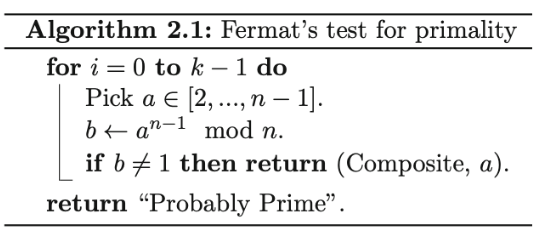
\includegraphics[scale=0.7]{img/fermatprimetest.png}
    \caption{Algorithm for Fermat Primality Test}
\end{figure}

\subsubsection{Miller-Rabin Primality Test}
The Miller-Rabin test is an improvement over the Fermat test. Unlike deterministic primality tests (which can definitively prove whether a number is prime), the Miller-Rabin test provides a result with high probability. If the test declares a number to be composite, then it is definitely not prime. However, if the test declares the number to be prime, there is still a small chance that it is actually composite (this is the ``probabilistic" part). The Miller-Rabin test checks whether a number $n$ passes certain conditions that hold for all prime numbers. It does this by examining the modular arithmetic properties of numbers related to $n$. If $n$ passes these tests, it is likely prime. If it fails, $n$ is definitely composite.

\begin{figure}[h!]
    \centering
    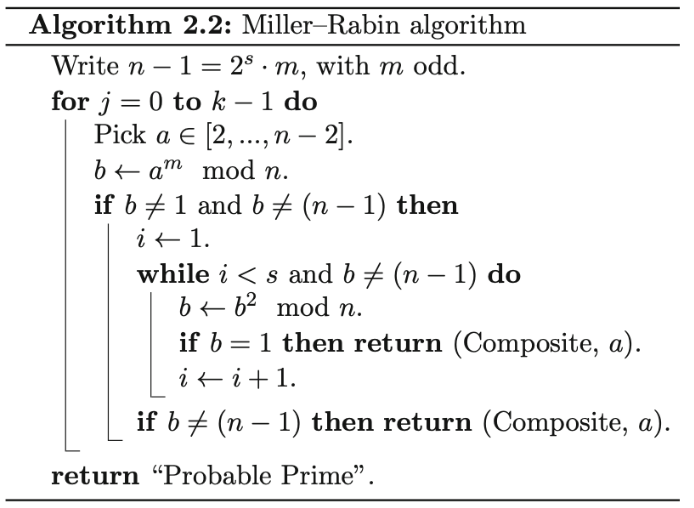
\includegraphics[scale=0.65]{img/MRprimetest.png}
    \caption{Algorithm for Miller-Rabin Test}
\end{figure}

% \begin{enumerate}
%     \item \textbf{Express \( n-1 \) as \( 2^s \cdot d \):}
%     \begin{itemize}
%         \item First, express \( n-1 \) as a product of a power of 2 and an odd integer. Specifically, find \( s \) and \( d \) such that:
%         \[
%         n-1 = 2^s \cdot d, \quad \text{where} \quad d \text{ is odd}.
%         \]
%         \item This can be done by repeatedly dividing \( n-1 \) by 2 until \( d \) becomes odd.
%     \end{itemize}

%     \item \textbf{Choose a random base \( a \):}
%     \begin{itemize}
%         \item Select a random integer \( a \) such that \( 1 < a < n-1 \).
%     \end{itemize}

%     \item \textbf{Compute \( a^d \mod n \):}
%     \begin{itemize}
%         \item Calculate \( a^d \mod n \) using modular exponentiation.
%     \end{itemize}

%     \item \textbf{Check the first condition:}
%     \begin{itemize}
%         \item If \( a^d \equiv 1 \pmod{n} \) or \( a^d \equiv n-1 \pmod{n} \), then \( n \) passes this round of the test.
%     \end{itemize}

%     \item \textbf{Iterate and square:}
%     \begin{itemize}
%         \item If neither of the above conditions hold, square \( a^d \mod n \) repeatedly \( s \) times (i.e., compute \( a^{2^i \cdot d} \mod n \) for \( i = 1, 2, \ldots, s-1 \)).
%         \item Check if any of these intermediate results equals \( n-1 \). If you find \( a^{2^i \cdot d} \equiv n-1 \pmod{n} \) for some \( i \), then \( n \) passes this round.
%     \end{itemize}

%     \item \textbf{Final check:}
%     \begin{itemize}
%         \item If \( n \) does not satisfy the conditions at any stage (i.e., if \( a^{2^i \cdot d} \mod n \neq 1 \) and \( a^{2^i \cdot d} \mod n \neq n-1 \) for all \( i \)), then \( n \) is composite.
%     \end{itemize}

%     \item \textbf{Repeat:}
%     \begin{itemize}
%         \item Repeat steps 2-6 with different random bases \( a \). Each round of testing reduces the probability of error.
%     \end{itemize}
% \end{enumerate}

\subsection{Elliptic Curves}
\begin{defn}
    An elliptic curve is an equation of the form $F: y^2 = x^3 + ax + b \mod p$, with constants a, b.
    \begin{itemize}
        \item $p > 3$, otherwise $x^3 = x$
        \item If P is on F, then also $P + P, P+P+P,$ ... are on F.
    \end{itemize}
\end{defn}

Not all equations make good elliptic curves. They must satisfy a condition that ensures there are no sharp points or self-intersections. The curve must be \emph{smooth} and \emph{non-singular}.
\[ 4a^3 + 27b^2 \neq 0 \]

\textbf{Point Addition:} 
\begin{itemize}
    \item Addition of two points $P$ and $Q$ on the curve gives you another point $R$, which is also on the curve. 
            To add \( P = (x_1, y_1) \) and \( Q = (x_2, y_2) \):
            \begin{enumerate}
                \item Draw a straight line through \( P \) and \( Q \). This line will generally intersect the curve at exactly one more point, say \( R' \).
                \item Reflect \( R' \) across the x-axis to get \( R = (x_3, y_3) \), the result of \( P + Q \).
            \end{enumerate}
            The formulas to compute \( R = (x_3, y_3) \) are:
            \[
            x_3 = \lambda^2 - x_1 - x_2
            \]
            \[
            y_3 = \lambda(x_1 - x_3) - y_1
            \]
            where \( \lambda \) (the slope of the line) is:
            \[
            \lambda = \frac{y_2 - y_1}{x_2 - x_1}
            \]
    \item If you’re adding $P$ to itself (doubling), the line you draw is the tangent to the curve at $P$.
    The formulas for \( R = 2P = (x_3, y_3) \) are:
    \[
    x_3 = \lambda^2 - 2x_1
    \]
    \[
    y_3 = \lambda(x_1 - x_3) - y_1
    \]
    Here, \( \lambda \) (the slope of the tangent) is:
    \[
    \lambda = \frac{3x_1^2 + a}{2y_1}
    \]
    \item If \( P \) and \( Q \) are vertical opposites (e.g., \( P = (x, y) \) and \( Q = (x, -y) \)), the line through them is vertical, and their sum is the \textbf{point at infinity}, \( \mathcal{O} \). Think of \( \mathcal{O} \) as the "zero" for point addition.
    \item Special properties:
    \begin{itemize}
        \item \textbf{Commutative:} \( P + Q = Q + P \)
        \item \textbf{Associative:} \( (P + Q) + R = P + (Q + R) \)
        \item \textbf{Identity Element:} Adding the point at infinity \( \mathcal{O} \) to any point \( P \) gives \( P \) (like adding zero).
    \end{itemize}
\end{itemize}

\begin{figure}[h!]
    \centering    
    \begin{subfigure}[b]{0.3\textwidth}
        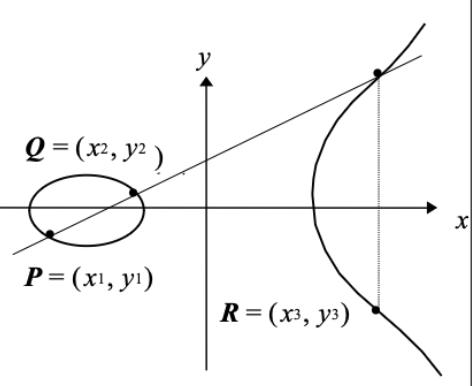
\includegraphics[width=\linewidth]{img/ecadd.png}
        \caption{Point Addition}
    \end{subfigure}
    \hfill
    \begin{subfigure}[b]{0.3\textwidth}
        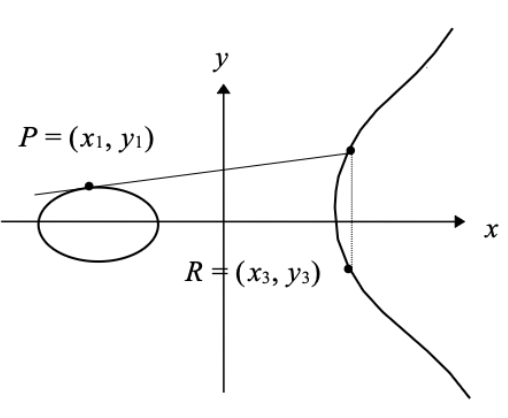
\includegraphics[width=\linewidth]{img/pointdoubling.png}
        \caption{Point Doubling}
    \end{subfigure}
    \hfill
    \begin{subfigure}[b]{0.3\textwidth}
        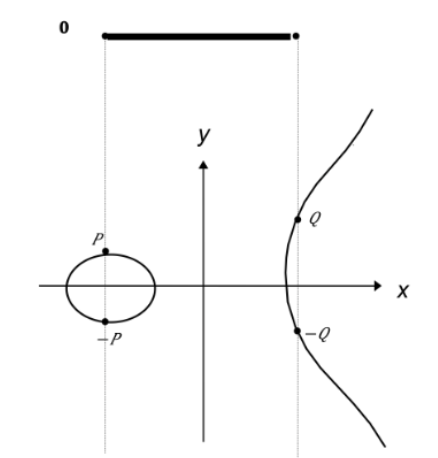
\includegraphics[width=\linewidth]{img/zeropoint.png}
        \caption{Zero Point}
    \end{subfigure}
\end{figure}

Using elliptic curves lets us create very secure systems with shorter keys (really large prime numbers are not required), which means faster and more lightweight encryption.

\begin{defn}
    \textbf{Elliptic Curve Discrete Log Problem}: For a given integer m and a point P, it is easy to compute $Q = mP$. However, given P and Q, it is hard to compute m.
\end{defn}

Imagine a simple operation: start at one point on the curve, "add" it to itself repeatedly, and you get another point. If I tell you the starting point and the number of additions, it's easy to figure out the end point. But if I give you the end point and ask you to figure out the number of additions, that's really hard. This is what makes elliptic curve cryptography (ECC) secure.

\section{Lecture 3}

\subsection{The Syntax of Encryption}

\subsection{Classical Ciphers}

\subsubsection{Caesar Cipher}

\subsubsection{Shift Cipher}

\subsubsection{Substitution Cipher}

\subsubsection{Vigenère Cipher}

\subsubsection{Permutation Cipher}


\section{Lecture 4}

\subsection{Security Definitions}
\begin{defn}
    Computationally Secure: it takes N operations using the \textbf{best known algorithm} to break a crytographic system and N is too large to be feasible.
\end{defn}

\begin{defn}
    Provably Secure: breaking the system is reduced to solving some well-studied hard problem.
\end{defn}

\begin{defn}
    Unconditional Secure/Perfectly Secure: the system is secure against an adversary with unlimited computational power.
\end{defn}

Key size is important. Advances in computer hardware and algorithms are important. In the future, it will be broken due to hardware or better algorithms.

\subsection{Probability and Ciphers}

\begin{defn}
Let $P$ denote the set of plaintexts, $K$ the set of keys, and $C$ denote the set of cipher texts. $p(P=m)$ is the probability that the plaintext is $m$. Then,
\[
p(C=c) = \sum_{k: c\in \mathbb{C}(k)} p(K=k)\cdot p(P=d_k(c))
\]
\end{defn}

\Comment{add examples in here}

\subsection{Perfect Secrecy}
Previously, the ciphertext revelas a lot of information about the plaintext. We want a system in which ciphertext does not reveal anything about the plaintext. 

\begin{defn}
    Perfect secrecy: a cryptosystem has perfect secrecy if \[ p(P=m | C=c) = p(P=m) \] for all plain texts $m$ and ciphertexts $c$.
\end{defn}

\begin{lem}
    Assume the cryptosystem is perfectly secure, then 
    \[ \#K \geq \#C \geq \#P\] where $\#$ denotes the number of items in the corresponding set. 
\end{lem}

\subsection{One-Time Pad}

\begin{thm}
    Shannon's Theorem: Let $(P, C, K, e_k(), d_k())$ denote a cryptosystem with \( \#K = \#C = \#P\). Then the cryptosystem provides perfect secrecy if and only if:
    \begin{itemize}
        \item Every key is used with equal probability $1/\#K$
        \item For each $m \in P$ and $c \in C$, there is a unique key $k$ such that $c = e_k(m)$
    \end{itemize}
\end{thm}

\Comment{Add modified shift cipher here}

\subsection{Entropy}
Due to the key distribution problem (the key must be as long as the message), perfect secrecy is not practical. Instead, we need a cryptosystem in which \textbf{one key can be used many times}, and \textbf{a  small key can encrypt a long message}. Such a system is not perfectly secure, but it should be computationally secure. We need to measure the amount of informatiomn first: Shannon's entropy. \\

\textbf{Example:} For a specific question X: ``Will you go out with me?'', the answer is Yes or No. If you always say No, the amount of information, $H(X) = 0$. If you always say Yes, $H(X) = 0$. You know the result. If you say Yes and No with equal probability, $H(X) = 1$. When you get the answer, no matter what it is, you learn a lot. Here, $H()$ is the entropy, and is independent of the length of $X$.

\begin{defn}
    Shannon's Entropy: Let $X$ be a random variable which takes a finite set of values $x_i$, with $1 \leq 1 \leq n$, and has a probability distribution $p(x)$. We use the convention that if $p_i = 0$ then $p_i \log_2(p_i) = 0$. The entropy of $X$ is defined as:

    \[ H(X) = -\sum_{i=1}^n p_i \cdot \log_2 p_i\] 

    Properties:
    \begin{itemize}
        \item $H(X) \geq 0$
        \item $H(X) = 0$ if $p_i = 1$ and $p_j = 0$ for $i \neq j$
        \item if $p_i = 1/n$ for all $i$, then $H(X) = \log_2(n)$
    \end{itemize}
\end{defn}

\subsection{Spurious Keys and Unicity Distance}


\end{document}